\documentclass[12pt, twoside]{article}
\usepackage[letterpaper, margin=1in, head=30pt, headsep=0.1in]{geometry}
\usepackage[english]{babel}
\usepackage[utf8]{inputenc}
\usepackage{amsmath}
\usepackage{amsfonts}
\usepackage{amssymb}
\usepackage{tikz}
\usepackage{yhmath} %arcs using \wideparen{}
\usetikzlibrary{quotes, angles}

\usepackage{graphicx}
\usepackage{enumitem}
\usepackage{multicol}

%\usepackage{pgfplots}
%\pgfplotsset{width=10cm,compat=1.9}
%\usepgfplotslibrary{statistics}
%\usepackage{pgfplotstable}
%\usepackage{tkz-fct}
%\usepackage{venndiagram}

\usepackage{fancyhdr}
\pagestyle{fancy}
\fancyhf{}
\renewcommand{\headrulewidth}{0pt} % disable the underline of the header
\raggedbottom
\newif\ifmeta
\metatrue %print standards and topics tags

\title{High School Geometry problem sets}
\author{Chris Huson}
\date{April 2021}

%\fancyhead[RE]{\thepage}
%\fancyhead[RO]{\thepage \\ Name: \hspace{3cm}}
%\fancyhead[L]{BECA / Dr. Huson / 10th Grade Geometry\\* 7 June 2019}
%
%\begin{document}
%\subsubsection*{13.7 Homework: Cross sections, distance applications}
%\fancyhead[L]{BECA / Dr. Huson / Geometry 03-Volume+angle-bisectors\\* pset ID: 34}

\begin{document}

\subsubsection*{8.3 Data visualization}
\begin{enumerate}
\item Do Now: Convert units of \emph{radians} and \emph{degrees} ($2 \pi = 360^\circ$, $\pi = 180^\circ$).\\[0.25cm]
  Apply the appropriate formula.
  \begin{multicols}{2}
    $\displaystyle d = r \times \frac{180}{\pi}$\\
    $\displaystyle r = d \times \frac{\pi}{180}$
  \end{multicols} \vspace{0.5cm}
  \begin{multicols}{2}
    \raggedcolumns
    \begin{enumerate}
      \item $\displaystyle m\angle A = \frac{\pi}{5}  =\hspace{0.15cm} ?$ degrees\\[0.75cm]
      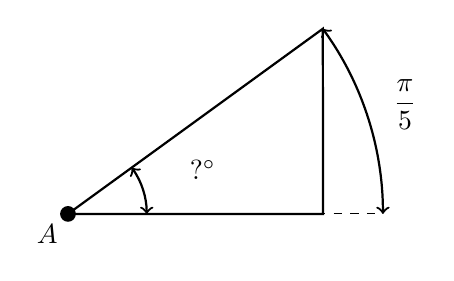
\begin{tikzpicture}[scale=1]
        \draw [thick, <->] (0:1) arc (0:36:1);
        \draw [thick, <->] (0:4) arc (0:36:4);
        \draw [dashed](0,0)--(4,0);
        \draw [thick]
        (0,0) node[below left] {$A$}--(36:4)--(3.24,0)--cycle;
        \fill (0,0) circle[radius=.1];
        \node at (18:1.8) {$?^\circ$};
        \node at (18:4.5) {$\displaystyle \frac{\pi}{5}$};
      \end{tikzpicture}
      \columnbreak
      \item $m\angle B = 60^\circ = \hspace{0.15cm} ?$ radians \\
      (in terms of $\pi$)\\[0.5cm]
      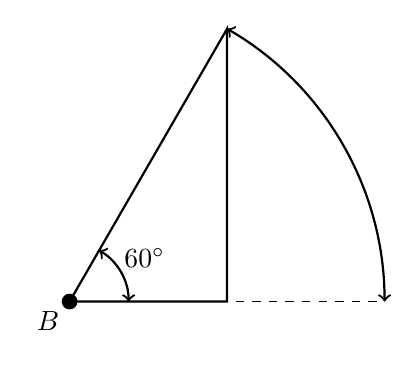
\begin{tikzpicture}[scale=1]
        \draw [thick, <->] (0:0.75) arc (0:60:0.75);
        \draw [thick, <->] (0:4) arc (0:60:4);
        \draw [dashed](0,0)--(4,0);
        \draw [thick]
        (0,0) node[below left] {$B$}--(60:4)--(2,0)--cycle;
        \fill (0,0) circle[radius=.1];
        \node at (30:1.1) {$60^\circ$};
      \end{tikzpicture}
    \end{enumerate}
  \end{multicols}

\newpage
\item Do Now: The \emph{pie chart} below shows the proportion of two subsets of a population, one represented in blue and one in orange. Dotted lines divide the circle in eight equal sectors for reference.
  \begin{multicols}{2}
  \raggedcolumns
  \begin{enumerate}[itemsep=1.5cm]
    \item Estimate the area of the blue sector as a fraction of the circle and as a decimal.
    \item The central angle of the orange sector measures $55^\circ$. Find the fraction of circle's area shaded orange as a fraction and a decimal.
  \end{enumerate}
  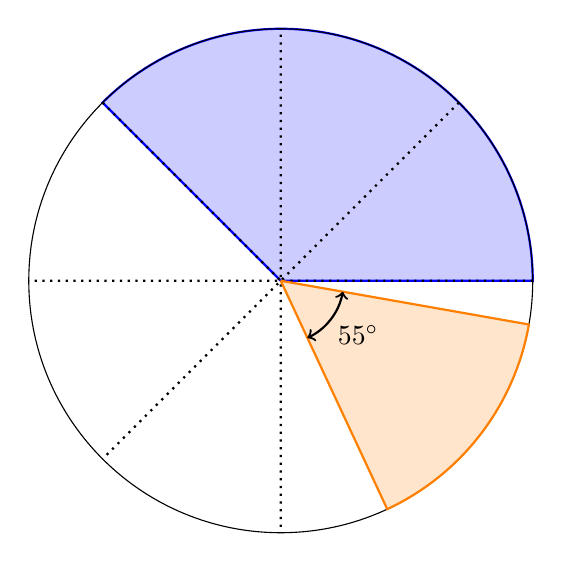
\begin{tikzpicture}[scale=0.8]
    \filldraw [color=blue, fill=blue!20, thick]
    (0,0)--(0:4) arc (0:135:4)--(0,0);
    \draw (0,0) circle[radius=4];
    %\draw [thick] (0:4) arc (0:36:4);
    %\draw [thick]
    %(0:4) node[right] {$A$}--
    %(0,0) node[below left] {$O$}--
    %(36:4) node[right] {$B$};
    \draw [thick, dotted](45:4)--(0,0)--(90:4);
    \draw [thick, dotted](135:4)--(0,0)--(180:4);
    \draw [thick, dotted](0:4)--(0,0)--(-135:4);
    \draw [thick, dotted](-45:4)--(0,0)--(-90:4);
    \filldraw [color=orange, fill=orange!20, thick]
    (0,0)--(-10:4) arc (-10:-65:4)--(0,0);
    \draw [thick, <->] (-10:1) arc (-10:-65:1);
    \node at (-35:1.5) {$55^\circ$};
  \end{tikzpicture}
  \end{multicols}

\newpage
\item Lesson: We use circle sectors (pie charts) to communicate. This map shows the most important of the 3991 coronavirus variants as they evolve across the world.
\begin{enumerate}[itemsep=0.7cm]
  \item In Europe, estimate the proportion of covid-19 identified as B.1.1.7 (light blue).
  \item In South America, which is more prevalent B.1.1.7 or P.1 (light orange)?
  \item In North America, what proportion of samples remain ``unassigned'' (gray)?
\end{enumerate}
  \begin{center}
    \includegraphics[width=18cm]{8-3Covid_map.png}
  \end{center}
  \begin{flushright}
    \includegraphics[width=5cm]{8-3Covid_map_legend.png}
  \end{flushright}
  %https://nextstrain.org/ncov/global?c=emerging_lineage&dmin=2020-12-21&p=full&r=region

\newpage
\item Groupwork: Compare the coronavirus variants across four states, regions, or countries.
\begin{enumerate}
  \item Screenshot a pie chart into your quadrant. Write down the most prevalent variant.
  \item Each student pastes a screenshot, name and region into each person's slide.
  \item Discuss the differences and similarities in your group and agree on two or three sentences you will all write (``Discussion'').
\end{enumerate}
\begin{center}
  \begin{tikzpicture}[scale=1, rotate=0]
  \draw [thick] (-5,0)--(5,0);
  \draw [thick] (0,-6)--(0,6);
  \node at (-4,6){Your name \& location:};
  \node at (3,6){Member name \& location:};
  \node at (3,-0.5){Member name \& location:};
  \node at (-4,-0.5){Member name \& location:};
\end{tikzpicture}
\end{center}
Discussion
%https://nextstrain.org/ncov/north-america?c=emerging_lineage&d=map,frequencies&dmin=2020-12-21&p=full&r=division
%https://covid.cdc.gov/covid-data-tracker/#variant-proportions

\newpage
\item Practice: Convert between units. \\[0.25cm]
General method: if $A = B$ multiply by $\displaystyle \frac{A}{B} \text{ or } \frac{B}{A}$. For example, $\pi \text{ radians}= 180 \text{ degrees}$ so \\
$\displaystyle r = d \times \frac{\pi}{180}$ and 
$\displaystyle d = r \times \frac{180}{\pi}$
\vspace{0.5cm}
  \begin{multicols}{2}
  \raggedcolumns
  \begin{enumerate}[itemsep=1.5cm]
    \item $40^\circ = \hspace{0.15cm} ?$ radians
    \item $\displaystyle \frac{\pi}{7}  = \hspace{0.15cm} ?$ degrees
    \item 1 foot = 12 inches\\[0.5cm]
    3.5 feet = 
    \item 54 inches = 
    \item 1 euro = 1.21 dollars\\[0.5cm]
    20 euro = 
    \item 100 dollars = 
    \item 1 mile = 5,280 feet\\[0.5cm]
    10,000 feet = 
    \item $\frac{1}{2}$ mile =   
  \end{enumerate}
  \end{multicols}


\end{enumerate}
\end{document}